\documentclass[11pt,letterpaper,titlepage]{article}

%================== Document nomenclature
\newcommand{\DOCSUBJT}{Personal Notes: }   %Put document subject here
\newcommand{\DOCTITLE}{                      %Put document title here
	Piece-wise linear shape/basis functions
}       
\newcommand{\DOCDATE} {August, 2018}         %Put document date here
\newcommand{\DOCREV}  {Rev 1.00}             %Put revision number here

%================== Misc Settings
\usepackage{fancyhdr}
\usepackage[left=0.75in, right=0.75in, bottom=1.0in]{geometry}
\usepackage{lastpage}
\usepackage{titleref}
\usepackage{booktabs}
\usepackage{appendix}

\appendixtitleon
\appendixtitletocon

\makeatletter

%================== List of figures and tables mods
\usepackage{tocloft}
\usepackage[labelfont=bf]{caption}

\renewcommand{\cftfigpresnum}{Figure\ }
\renewcommand{\cfttabpresnum}{Table\ }

\newlength{\mylenf}
\settowidth{\mylenf}{\cftfigpresnum}
\setlength{\cftfignumwidth}{\dimexpr\mylenf+1.5em}
\setlength{\cfttabnumwidth}{\dimexpr\mylenf+1.5em}



%=================== Graphics
\usepackage{graphicx}
\usepackage[breakwords]{truncate}
\usepackage{float}
\usepackage{array}
\usepackage{amsmath}
\usepackage{mdframed}
\usepackage{fancyvrb}
\usepackage{float}
\usepackage{cancel}
\usepackage{amssymb}
\graphicspath{ {images/} }
\usepackage[usenames,dvipsnames,svgnames,table]{xcolor}
\usepackage[defaultlines=2,all]{nowidow}
\usepackage{listings}
\usepackage{color}
\definecolor{Brown}{cmyk}{0,0.81,1,0.60}
\definecolor{OliveGreen}{cmyk}{0.64,0,0.95,0.40}
\definecolor{CadetBlue}{cmyk}{0.62,0.57,0.23,0}
\usepackage{pdflscape}
\usepackage{relsize}
\usepackage{verbatim}
\usepackage{tabto}
%\usepackage{upgreek}
\usepackage{enumitem}
\usepackage{pstricks}
\usepackage{pstricks-add}
\usepackage{pst-grad}
\usepackage{pst-plot}
\usepackage{geometry}
\usepackage{pst-tools}

%\usepackage{MnSymbol}% http://ctan.org/pkg/mnsymbol

%=================== Big cdot
\newcommand*\bigcdot{\mathpalette\bigcdot@{.5}}
\newcommand*\bigcdot@[2]{\mathbin{\vcenter{\hbox{\scalebox{#2}{$\m@th#1\bullet$}}}}}

%=================== Settings
\renewcommand{\baselinestretch}{1.2}
\definecolor{gray}{rgb}{0.4 0.4 0.4}
\newcommand{\stimes}{{\times}}

%================== Code syntax highlighting
\lstset{language=C++,frame=ltrb,framesep=2pt,basicstyle=\linespread{0.8} \small,
	keywordstyle=\ttfamily\color{OliveGreen},
	identifierstyle=\ttfamily\color{CadetBlue}\bfseries,
	commentstyle=\color{Brown},
	stringstyle=\ttfamily,
	showstringspaces=true,
	tabsize=2,}
	
%================== Section numbers with equation numbers
\numberwithin{equation}{section}

%================== Short \to arrow
\setlength{\medmuskip}{0mu}
%\newcommand{\tos}[1][3pt]{\mathrel{%
%   \hbox{\rule[\dimexpr\fontdimen22\textfont2-.2pt\relax]{#1}{.4pt}}%
%   \mkern-4mu\hbox{\usefont{U}{lasy}{m}{n}\symbol{41}}}}





\begin{document}

\begin{titlepage}
	\pagestyle{fancy}
	\vspace*{1.0cm}
	\centering
	\vspace{1cm}
	\vspace{.25cm}
	{\Large\bfseries  \DOCSUBJT \par} 
	{\Large\bfseries \DOCTITLE  \par}
	\vspace{1cm}
	{\Large \DOCDATE \par}
	\vspace{1.0cm}
	{\Large Jan Vermaak \par}
	{\Large \DOCREV \par}

\end{titlepage}	


\pagestyle{fancy}
\rfoot{Page \thepage \ of \pageref{LastPage}}
\cfoot{}
\lfoot{\truncate{14cm}{\DOCTITLE}}
\rhead{}
\chead{\currentname}
\lhead{}
\renewcommand{\footrulewidth}{0.4pt}
\setlength\parindent{0pt}
\begin{comment}
\tableofcontents
\addtocontents{toc}{~\hfill\textbf{Page}\par}

\listoffigures
\listoftables

\end{comment}
\chead{Contents}	

%#########################################################################
\newpage
\chead{Two Dimensional Triangle}
\section{Fundamental strategy}
In the finite element method the basic poisson equation,
\begin{align*}
-\nabla^2 \phi + \sigma_a \phi = q,
\end{align*}
is multiplied by a trial function $v_i$ to obtain

\begin{align*}
-\int_V v_i \nabla^2 \phi.dV + \int_V v_i.\sigma_a \phi.dV = \int_V v_i.q .dV.
\end{align*}
We then integrate by parts
\begin{align*}
-\int_V \nabla (v_i \nabla \phi).dV + \int_V  \nabla v_i \bigcdot \nabla \phi.dV
+ \int_V v_i.\sigma_a \phi.dV = \int_V v_i.q .dV
\end{align*}
and apply Gauss' divergence theorem to get
\begin{align*}
-\int_S \mathbf{\hat{n}}\bigcdot (v_i \nabla \phi).dA + \int_V \nabla v_i \bigcdot\nabla \phi.dV
+ \int_V v_i.\sigma_a \phi.dV = \int_V v_i.q .dV
\end{align*}
We then expand $\phi$ into basis functions and coefficients $\phi=\sum \phi_j b_j$ after which we get

\begin{align*}
\sum_j
-\int_S \mathbf{\hat{n}}\bigcdot (v_i \phi_j \nabla b_j).dA + \int_V \phi_j\nabla v_i \bigcdot\nabla b_j.dV
+ \int_V \phi_j \sigma_a v_i.b_j.dV = \int_V v_i.q .dV
\end{align*}

The goal of this exercise is to define the trial functions $v_i$ and basis functions $b_j$

\newpage
\section{Two Dimensional Triangle}
We start with the two dimensional reference triangle as shown in Figure \ref{fig:twodnatruralcoords} below. We wish to map any triangular cell $C$ to this reference triangle in order to develop a consistent method for item_id of any orientation.

\begin{figure}[h]
	\centering
	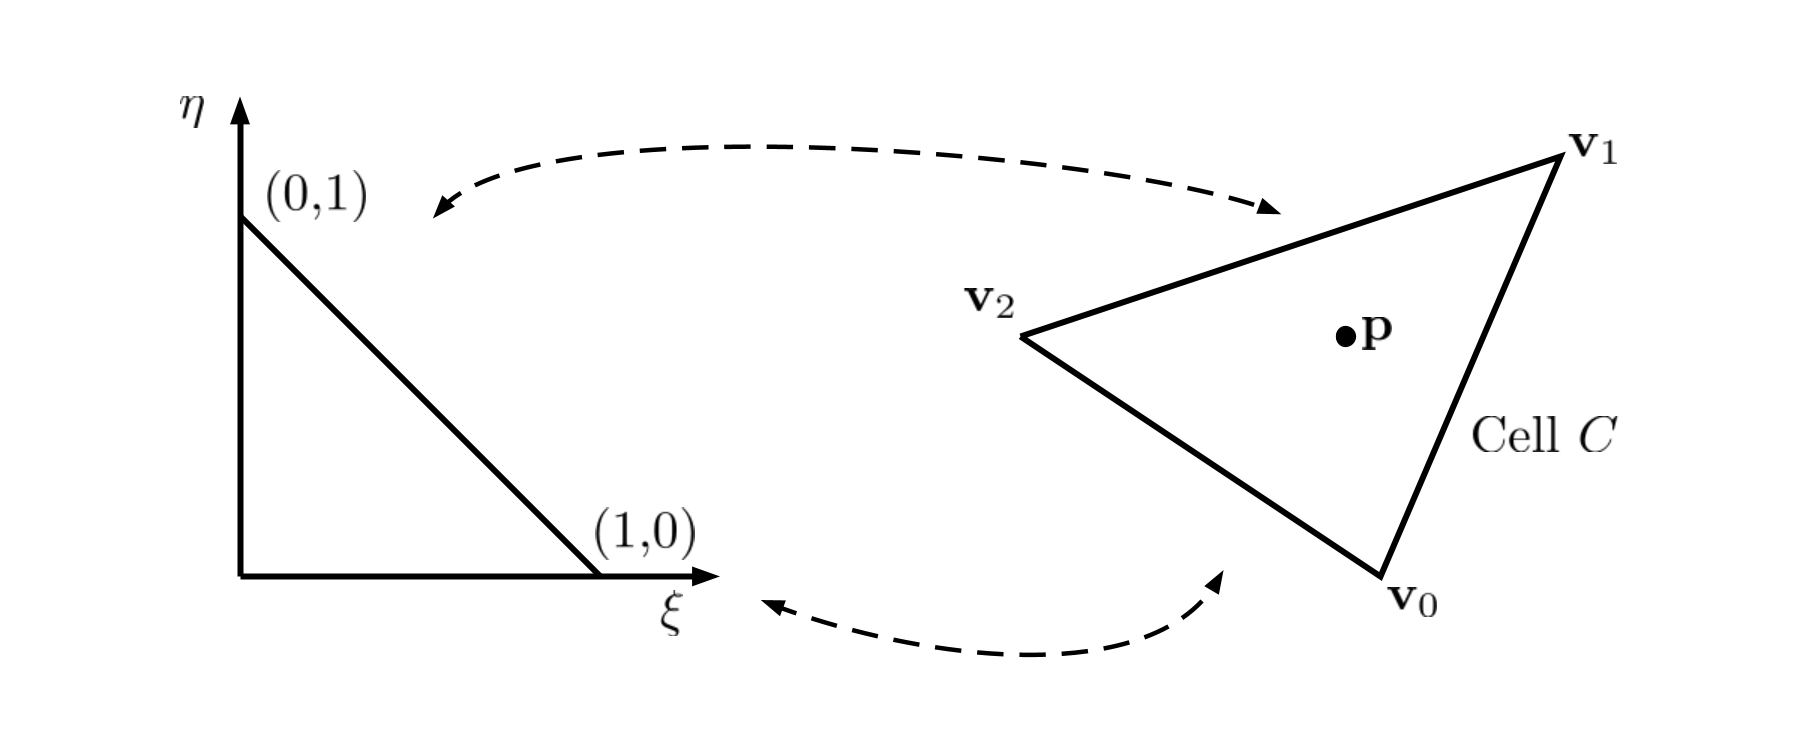
\includegraphics[width=0.7\linewidth]{Images/TwoDNatruralCoords}
	\caption{Natural coordinates used as a reference 2D element.}
	\label{fig:twodnatruralcoords}
\end{figure}

We first see that we can project any point $\textbf{p}{=}(x,y)$, within $C$, using a set of dot products
\begin{align}
\xi = (\textbf{p}-\textbf{v}_0) {\bigcdot} (\textbf{v}_1-\text{v}_0) \\
\eta = (\textbf{p}-\textbf{v}_0) {\bigcdot} (\textbf{v}_2-\text{v}_0).
\end{align}
Conversely we can map any point, in the natural coordinates triangle, to a point in $C$ as
\begin{align}
\textbf{p} = \textbf{v}_0 + \xi (\textbf{v}_1-\textbf{v}_0) + \eta  (\textbf{v}_2-\textbf{v}_0).
\end{align}
In expanded form this is
\begin{align*}
x = \text{x}_0 + \xi (\text{x}_1-\text{x}_0) + \eta  (\text{x}_2-\text{x}_0) \\
y = \text{y}_0 + \xi (\text{y}_1-\text{y}_0) + \eta  (\text{y}_2-\text{y}_0) 
\end{align*}
from which we determine 
\begin{align*}
\frac{\partial x}{\partial \xi} = \text{x}_1-\text{x}_0 
\quad \quad
\frac{\partial x}{\partial \eta} = \text{x}_2-\text{x}_0 \\
\frac{\partial y}{\partial \xi} = \text{y}_1-\text{y}_0 
\quad \quad
\frac{\partial y}{\partial \eta} = \text{y}_2-\text{y}_0. 
\end{align*}
We can then define the Jacobian matrix of the transformation
\begin{align}
J = 
\begin{bmatrix}
\dfrac{\partial x}{\partial \xi} & \dfrac{\partial x}{\partial \eta} \\
\dfrac{\partial y}{\partial \xi} & \dfrac{\partial y}{\partial \eta}
\end{bmatrix}
=
\renewcommand*{\arraystretch}{1.5}
\begin{bmatrix}
\text{x}_1-\text{x}_0 & \text{x}_2-\text{x}_0 \\
\text{y}_1-\text{y}_0 & \text{y}_2-\text{y}_0
\end{bmatrix}
\end{align}
which gives us the simplified form 

\begin{align}
\begin{bmatrix}
x \\ 
y
\end{bmatrix}
=
\begin{bmatrix}
x_0 \\ 
y_0
\end{bmatrix} 
+ J
\begin{bmatrix}
\xi \\ 
\eta
\end{bmatrix}
\end{align}
and
\begin{align}\label{eq:2dmap_nat_to_cart}
\begin{bmatrix}
\xi \\ 
\eta
\end{bmatrix}
=J^{-1}
\begin{bmatrix}
x -x_0\\ 
y -y_0
\end{bmatrix}.
\end{align}
For a $2{\times}2$ matrix the inverse of the Jacobian, $J^{-1}$, can easily be determined as
\begin{align}
J^{-1}=\dfrac{1}{|J|}
\begin{bmatrix}
\ \dfrac{\partial y}{\partial \eta} &-\dfrac{\partial x}{\partial \eta} \\
-\dfrac{\partial y}{\partial \xi} & \ \dfrac{\partial x}{\partial \xi}
\end{bmatrix}
\end{align}
We can now define a basis function $\bar{b}$ for each vertex of the reference triangle 
\begin{equation}
\begin{aligned}
\bar{b}_0(\xi,\eta) &= 1-\xi -\eta \\
\bar{b}_1(\xi,\eta) &= \xi\\
\bar{b}_2(\xi,\eta) &= \eta 
\end{aligned}
\end{equation}
and map it to cartesian coordinates to find

\begin{equation}
\begin{aligned}
b_0(x,y) &= 1 - J_{11}^{-1}(x - x_0) - J_{12}^{-1}(y-y_0)- J_{21}^{-1}(x - x_0) - J_{22}^{-1}(y-y_0) \\
b_1(x,y) &=J_{11}^{-1}(x - x_0) + J_{12}^{-1}(y-y_0) \\
b_2(x,y) &=J_{21}^{-1}(x - x_0) + J_{22}^{-1}(y-y_0).
\end{aligned}
\end{equation}
\newline

\subsection{Integrating the basis functions}
The finite element method will in some form require the integration of the basis functions over either a volume or an area. Integrating the basis functions over an area can be accomplished as 
\begin{align*}
\int \int b_j(x,y).dx.dy = \int \int \bar{b}_j .|J|.d\xi.d\eta.
\end{align*}
This integration involves linear functions for which we can use a quadrature rule.

\subsection{Integrating the gradient of the basis functions}


In any finite element method there would be the need for the integration of the shape functions as well as the gradients of the shape functions. The shape functions are now already defined in this context but we still need the gradients of the shape functions

\begin{align*}
\vec{\nabla}f = 
\renewcommand*{\arraystretch}{1.8}
\begin{bmatrix}
\dfrac{\partial f}{\partial x} \\
\dfrac{\partial f}{\partial y}
\end{bmatrix}
\end{align*}
Now from the chain rule we have
\begin{align*}
\renewcommand*{\arraystretch}{1.8}
\dfrac{\partial f}{\partial x} 
= \dfrac{\partial f}{\partial \xi}    \dfrac{\partial \xi}{\partial x}
+ \dfrac{\partial f}{\partial \eta}    \dfrac{\partial \eta}{\partial x} \\
\dfrac{\partial f}{\partial y} 
= \dfrac{\partial f}{\partial \xi}    \dfrac{\partial \xi}{\partial y}
+ \dfrac{\partial f}{\partial \eta}    \dfrac{\partial \eta}{\partial y}
\end{align*}
Which we can write as
\begin{align*}
\renewcommand*{\arraystretch}{1.8}
\begin{bmatrix}
\dfrac{\partial f}{\partial x} \\
\dfrac{\partial f}{\partial y}
\end{bmatrix}
=
\begin{bmatrix}
\dfrac{\partial \xi}{\partial x}     &\dfrac{\partial \eta}{\partial x} \\
 \dfrac{\partial \xi}{\partial y}    &\dfrac{\partial \eta}{\partial y}
\end{bmatrix}
\begin{bmatrix}
\dfrac{\partial f}{\partial \xi} \\
\dfrac{\partial f}{\partial \eta}
\end{bmatrix}
\end{align*}
But recall the mapping in equation \ref{eq:2dmap_nat_to_cart} for which we have
\begin{align*}
\xi &= J_{11}^{-1} (x-x_0)+J_{12}^{-1} (y-y_0) \\
\eta &= J_{21}^{-1} (x-x_0)+J_{22}^{-1} (y-y_0)
\end{align*}
Therefore
\begin{align*}
\renewcommand*{\arraystretch}{1.8}
\begin{bmatrix}
\dfrac{\partial f}{\partial x} \\
\dfrac{\partial f}{\partial y}
\end{bmatrix}
=
J^{-1}
\begin{bmatrix}
\dfrac{\partial f}{\partial \xi} \\
\dfrac{\partial f}{\partial \eta}
\end{bmatrix}
\end{align*}

\newpage
\section{Polygon}

\begin{figure}[h]
	\centering
	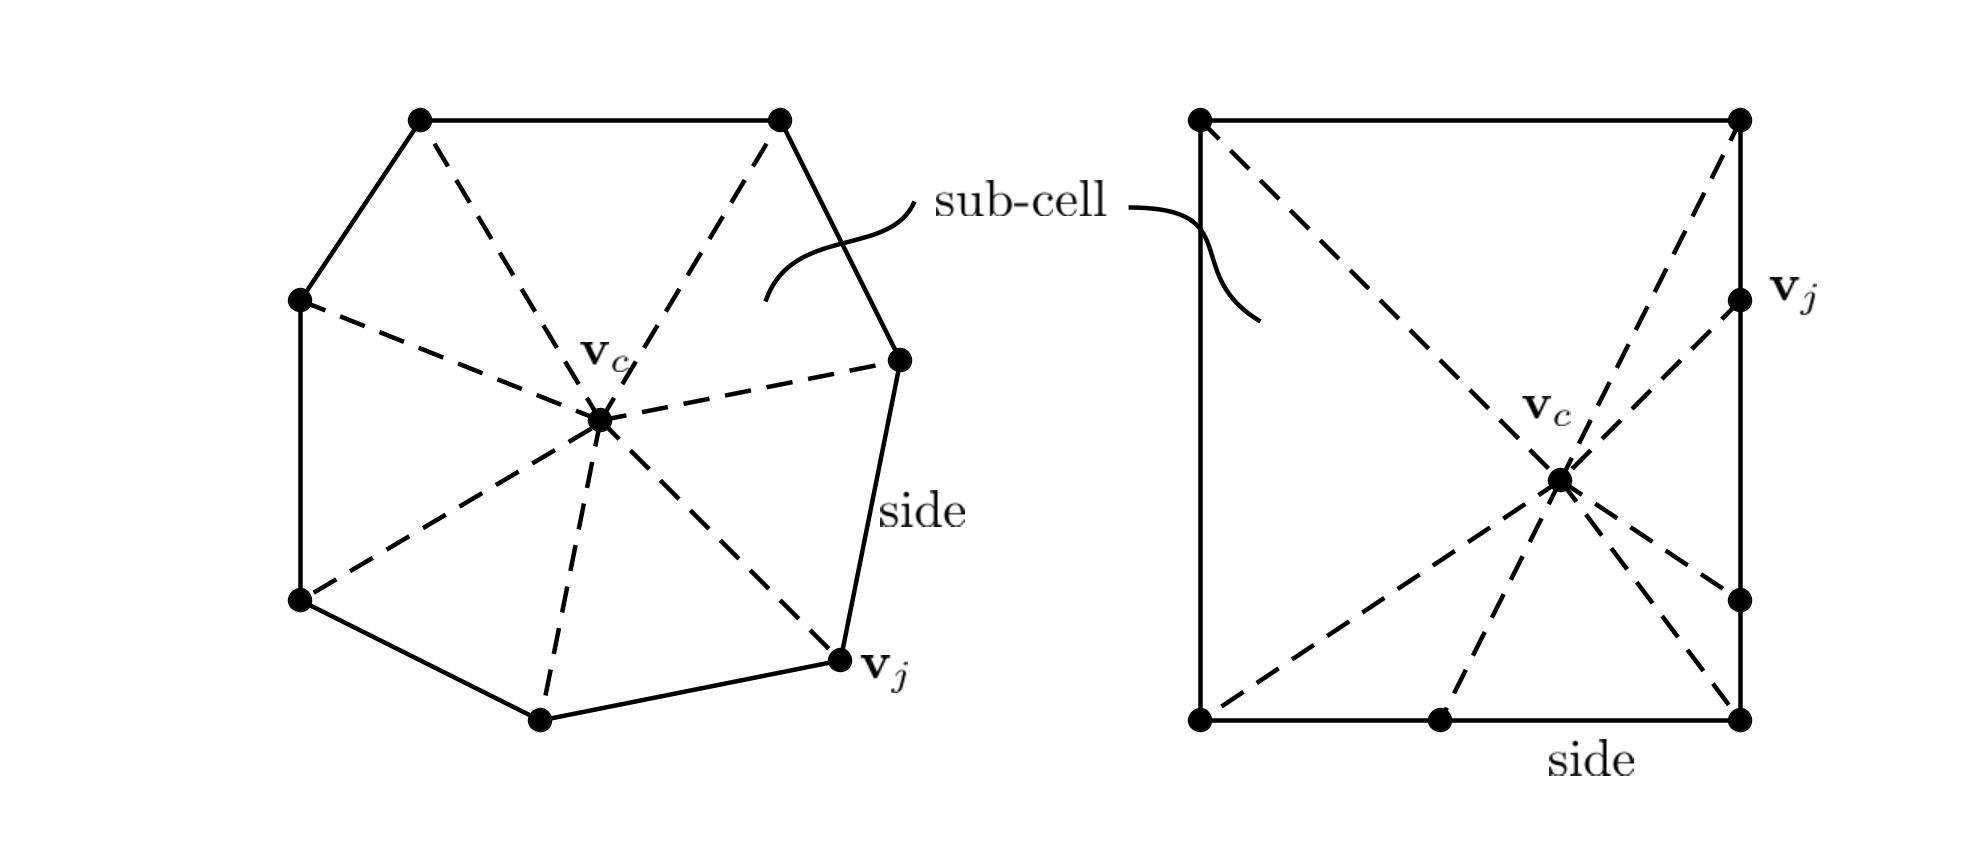
\includegraphics[width=0.7\linewidth]{Images/Polygon}
	\caption{Application of sub-item_id for polygons}
	\label{fig:polygon}
\end{figure}






\newpage
\begin{appendices}
\vspace{1cm}

\end{appendices}

\newpage
\chead{References}
\begin{thebibliography}{1}
    
    \bibitem{blender} {\em Blender - a 3D modelling and rendering package}, Blender Online Community, Blender Foundation, Blender Institute, Amsterdam, 2018
    
    \bibitem{delaunay} Cheng et al, {\em Delaunay Mesh Generation}, Chapman \& Hall/CRC Computer \& Information Science Series, 2013
    
    
\end{thebibliography}





\end{document}